\graphicspath{{imgs/}}
\documentclass[main.tex]{subfiles}
\begin{document}
\chapter{Results}\label{chap:results}
This chapter presents the result of the training process. The final network performances are evaluated and compared to other papers. The network's extracted features are further analyzed and a way forward is sketched.

\section{The trained Network}
The used model is inspired by the network presented in \cite{huang2017lung} and performs with a sensitivity of around 81$\%$ on the validation set and a false positive rate of $0.192$ per sample. This is already a better result than Xu et al.~\cite{xu1997development}, Armato et al.~\cite{armato1999computerized}, Lee et al.~\cite{lee2001automated}, Suzuki et al.~\cite{suzuki2003massive} and Teramoto et al.~\cite{teramoto2013fast} approaches.

todo: explain why that might not be the most relevant perf number


\begin{figure}
\begin{center}
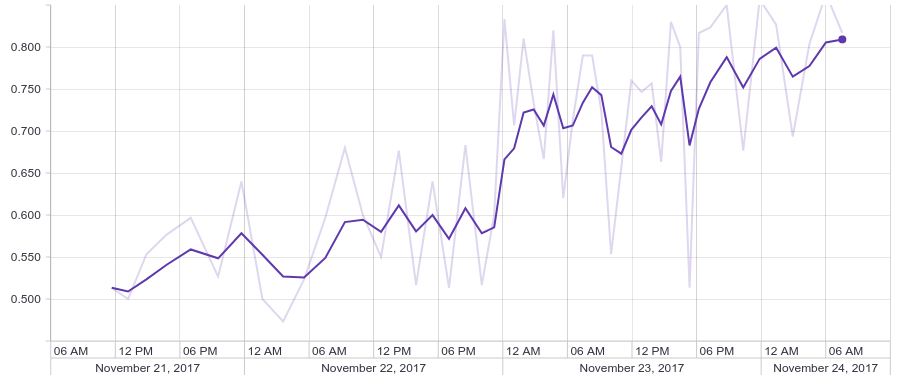
\includegraphics[scale=0.5]{validation_process.png}
\end{center}
\caption{Learning process of the network - the graph shows the developement of the accuracy of the network on the validation set. The darker line represents the smoothed values of the lighter line. Since the training is performed on the CPU (GPU can not be utilized since the network was too big.), it takes several days.}
\label{fig:validation}
\end{figure}


\section{Analyzing the Network}
To understand how a network solves the task it makes sense to look at the patterns it's layers a sensitive to. The convolutional layers allow for visual inspection.
Focus on the conv layers, what do they look like? Any hint on the geometry they are sensitive to?
Activation patterns to synthetic data and patches from the patients.

How is that best understood? 2 Approaches: first mean activation of the filters in each layer per img.

\subsection{Mean Class Activation}

\begin{figure}
\begin{center}
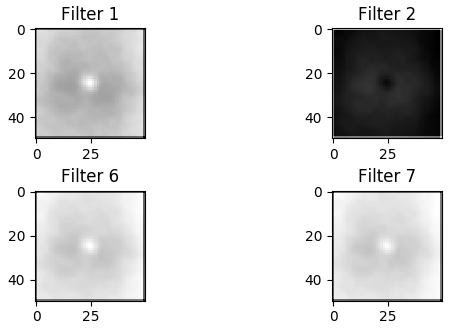
\includegraphics[scale=0.5]{nodule_activation_example.png}
\end{center}
\caption{The mean activation from 500 nodule patches of the validation set. Already in the first layer is the receptive field focusing on the center area, where the nodule resides.}
\label{fig:mean_activation}
\end{figure}


\section{Bridge to other Approaches}
How could a comparison at all be achieved? What is hindering the straightforward comparison of the kernel weights? Draw out a method to do that
Show what has been done
Compare performance to hand crafted approaches, 
take numbers out of papers

what could be similar features in the network?
\end{document}